% Para iniciar una sección debe escribirse
%\section{Nombre de la sección}
% Lo anterior inmediatamente creará la sección y la numerará.

\section*{Objetivos}
\subsection*{Generales}
\begin{itemize}
    \item Diseñar y construir un circuito secuencial capaz de controlar dos semáforos de una intersección, con la ayuda de sensores
\end{itemize}

\subsection*{Específicos}
\begin{itemize}
    \item Diseñar múltiples circuitos secuenciales para obtener un resultado único en conjunto
    \item Implementar un circuito de lógica secuencial capaz de realizar operaciones predefinidas a través de una Máquina de Estados Finitos (FSM)
    \item Contrastar los diseños teóricos con los resultados experimentales de los circuitos implementados físicamente
\end{itemize}

% \section{Introducción}

% \subsection{Aritmética binaria}
% Los dispositivos digitales se basan en operaciones con numeración \emph{base 2} para obtener los resultados, incluso si la interfaz de usuario tuviese otro 
% formato (numérico decimal, en base a gráficos o imágenes, etc.). Las operaciones aritméticas en \emph{base 2} cumplen con los mismos teoremas y reglas que se
% utilizan en base 10, pero poseen la ventaja de tener más simplificaciones debido a la limitada cantidad de dígitos disponibles. Consulte su libro de
% texto\footnote{Mano, Morris. Digital Design, 5th edition} para recapitular lo anteriormente descrito.

% \pagebreak

\section{Desarrollo Experimental}
\subsection{Materiales y Equipo}

Cada grupo debe llevar su material y equipo de trabajo durante las prácticas. Pregunte a su profesor qué \emph{Equipo de Laboratorio} puede ser prestado
de parte del laboratorio de instrumentación. El laboratorio de instrumentación no tiene disponibilidad de ningún elemento de la lista \emph{Materiales}.

\subsubsection*{Materiales}
\begin{itemize}
    \item 3x pulsadores
    \item 1x interruptor SPST (o un pulsador de enclave)
    \item 1x fuente de alimentación (ver apartado anterior con todas las alternativas)
    \item 2x capacitores electrolíticos de 47 $\mu$F 16V
    \item 2x capacitores cerámicos de 100nF 25V
    \item 2x resistencias de 1 k$\ohm$
    \item 2x LEDs verdes
    \item 2x LEDs rojos
    \item 2x LEDs amarillos
    \item 6x Resistencias $220 \ohm \leq R \leq 1 k\ohm$
    \item 2x Resistencias para temporización de reloj
    \item 1x Capacitor para temporización de reloj
    \item 1x Capacitor $10nF \leq C \leq 100nF$
    \item 1x circuito integrado temporizador 555
    \item Flip-flops de acuerdo a su diseño (se recomienda 74LS175 si en su diseño utiliza FFs tipo D)
    \item Las compuertas lógicas a utilizar dependen del diseño final de cada grupo (AND, OR, NOT, XOR, NAND, XNOR)
    \item 6x metros de alambre para protoboard calibre 22. Compren al menos 2 colores para los 6 metros. \textbf{No usen \emph{UTP}}, aunque eso les quieran vender.
\end{itemize}


\subsubsection*{Equipo de Laboratorio}
\begin{itemize}
    \item 1x Pinzas delgadas
    \item 1x Cortaalambres
    \item 1x Pelador de alambres para calibre 22 (opcional)
    \item 1x Tijeras pequeñas o cortauñas (si no tienen pela alambres)
    \item 1x Protoboard de al menos 2 galletas (puede juntar 2 protoboards de 1 galleta)
    \item 1x Multímetro digital para medir voltaje
\end{itemize}

\subsection{Procedimiento}
\subsubsection{Fuente de alimentación}
Utilice la misma fuente de alimentación que en la Práctica \#1.

\subsection{Reloj del sistema}
Diseñe un reloj de frecuencia constante y ciclo de trabajo cercano al 50\% para controlar la lógica combinacional del proyecto. Utilice un temporizador 555 haciendo uso de las 
ecuaciones de diseño en modo astable. Tome en cuenta que para el diseño del semáforo cada ciclo de reloj puede significar un cambio de estado, por lo que el período de cada pulso
de reloj debe rondar la \emph{escala humana} (más de 5 segundos, por ejemplo).

\subsubsection{Semáforos en intersección}
Se debe diseñar la lógica necesaria para manejar 2 semáforos: el primero ubicado en una avenida (vía principal) y el segundo ubicado en la calle que atraviesa la avenida.
El sistema debe funcionar dando prioridad \emph{en verde} a la avenida. Debajo del asfalto hay un sensor inductivo (uno debajo de la avenida y uno debajo de la calle) capaz
de detectar la presencia de tráfico en espera (este sensor será simulado con un pulsador). Ver Figura \ref{Fig:Semaforos} para más detalles.

El sistema de semáforos controla el tráfico de vías muy transitadas, por lo que no es posible que éste deje de funcionar súbitamente tras un fallo en el suministro de energía eléctrica.
Para subsanar esta situación existe una batería de respaldo, pero deberá indicarse a los conductores que el semáforo está en riesgo de apagarse: entrando en modo de advertencia.

El modo de advertencia consiste en hacer parpadear en amarillo el semáforo de la avenida y parpadear en rojo el semáforo de la calle hasta el instante que se restaure el 
suministro eléctrico.

\begin{figure}[H]
    \centering
    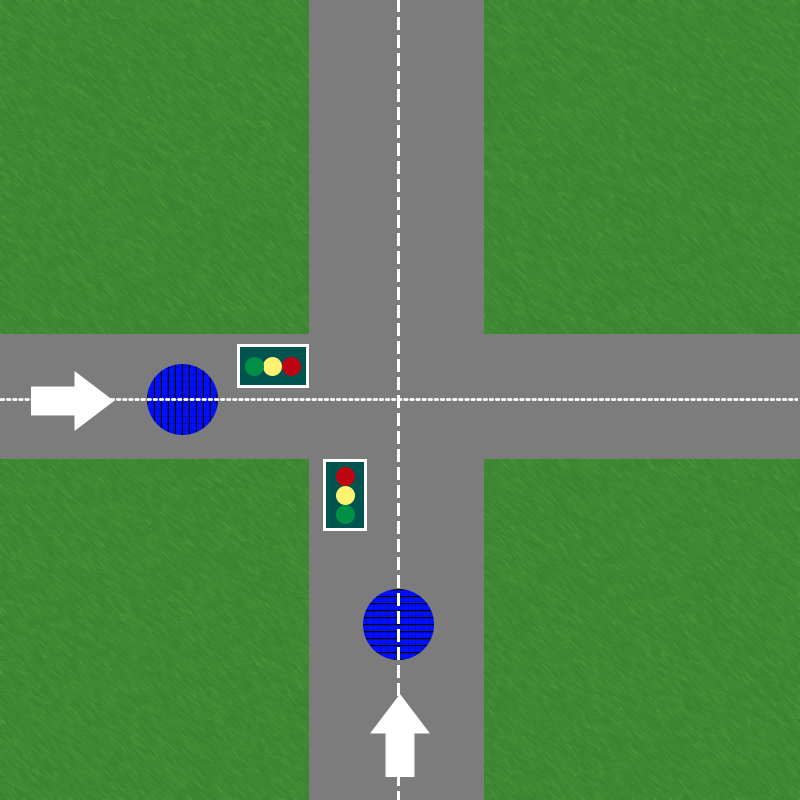
\includegraphics[scale=0.4]{images/Semaforos.png}
    \caption{Esquema de sistema de semáforos con sensores}
    \label{Fig:Semaforos}
\end{figure}

\subsection{Interfaz de usuario}
El usuario simulará algunas de las situaciones hipotéticas. No es necesario hacer una maqueta, pero al menos deben colocar ordenadamente los dispositivos de interfaz de usuario de tal forma
que se entienda a qué parte del circuito pertenece cada uno de éstos. Para la interfaz de salida se utilizarán los LEDs, uno de cada color, para cada uno de los semáforos. Para la 
interfaz de entrada se simularán las siguientes condiciones:

\begin{itemize}
    \item Sensor de presencia de automovil en calle o avenida: pulsador
    \item Corte de energía eléctrica: interruptor de enclave
\end{itemize}  

\subsection{Bonus}
Debido a la frecuencia baja del reloj del sistema, el usuario debe mantener presionado el push-button que simula a cualquiera de los sensores hasta el siguiente ciclo de reloj.
Para evitar esto, es posible diseñar un circuito basado en 555 que cuando se detecte una pulsación, este genere una salida única en alto de tiempo constante que se asegura se
mantena activa durante al menos (y no más de) 1 ciclo de reloj. En todo caso, debería implementarse un circuito \textbf{Monostable} con 555 para cada pulsador. Como compensación
se retribuirían 10 pts del primer examen parcial.